\documentclass[tikz,border=10pt]{standalone}
\begin{document}
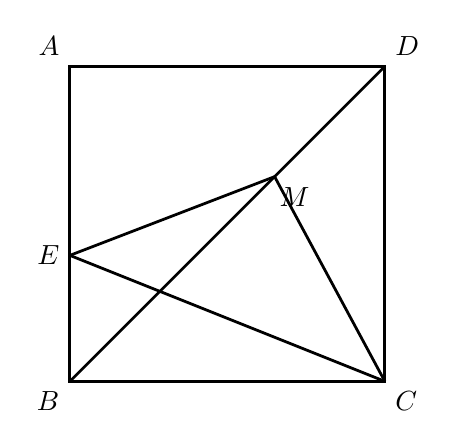
\begin{tikzpicture}[line width=1pt]
\coordinate (A) at (0,4);
\coordinate (B) at (0,0);
\coordinate (C) at (4,0);
\coordinate (D) at (4,4);
\coordinate (E) at (0,1.6);
\coordinate (M) at (2.6,2.6);

\draw (A) -- (B) -- (C) -- (D) -- cycle;
\draw (B) -- (D);
\draw (E) -- (M);
\draw (E) -- (C);
\draw (M) -- (C);

\node[above left] at (A) {$A$};
\node[below left] at (B) {$B$};
\node[below right] at (C) {$C$};
\node[above right] at (D) {$D$};
\node[left] at (E) {$E$};
\node[below right, xshift=-2pt] at (M) {$M$};
\end{tikzpicture}
\end{document}
